\chapter{A-Train}
\textit{A-Train}, also called the `\textit{Afternoon constellation}', is a formation of five
polar-orbiting
satellites, one of which was launched by the French space research agency
CNES, and the remainder were launched as part of NASA EOS (Earth Observing
System) and NASA ESPP (Earth
System Science Pathfinder) missions.
The primary focus of the constellation is to provide observations of clouds and
aerosols which would not be possible from ground-based or airborne
applications.
Aqua, the first member of the constellation, was launched in~2002, followed by
Aura and PARASOL in~2004, and CloudSat and CALIPSO in~2006
\citep{A-TrainFactsheet2003, TheEarthObserverJun2006}. The group was to be
joined by OCO (Orbiting Carbon Observatory) in~2009; however, the satellite
failed to make orbit and disintegrated in the atmosphere
\citep{OCO_NatureGeoscienceApr2006}.
Fig.~\ref{fig:atrain-overview} gives a simplistic view of the constellation.

\begin{figure}[h]
\includegraphics[width=\textwidth]{images/atrain-overview.jpg}
\caption[A not-to-scale overview of the A-Train constellation]{\textbf{A not-to-scale overview of the A-Train constellation.} Listed
under the track is the approximate temporal separation. Note that as a
result of launch failure, OCO is not in the constellation. [Adapted from
\url{
http://www.nasa.gov/mission_pages/cloudsat/multimedia/a-train.html}.]}
\label{fig:atrain-overview}
\end{figure}

The satellites fly on a 705-km sun-synchronous retrograde orbit at an
inclination of \ang{98},
and velocity of about \SI{7}{km.s^{-1}}.
The leading and trailing members are
separated by approx.~\SI{15}{min}. The formation is dubbed `\textit{afternoon}',
because it
crosses the
equator at 1:30\,pm local mean time, circulating around the Earth 14.56~times
per \SI{24}{h} \citep{CloudSatHandbook2008}. The A-Train travels northward
during the day half-orbit, and southward during the night half-orbit. The leading
satellite Aqua repeats its ground track every 16~days. CloudSat is
maneuvered to
maintain a maximum of \SI{15}{s} along-track distance from CALIPSO, which itself
is
configured to lag Aqua by no more than \SI{120}{s}
\citep{CALIPSO_CloudSat_GRACE_ScienceWritersGuide2005}. Such proximity means
that data from a diversity of
instruments can easily be combined together.
The instruments covered here are the CALIOP lidar on CALIPSO, the millimetre-wave radar CPR on
CloudSat and the passive spectroradiometer MODIS carried on-board of Aqua.

\begin{figure}[t]
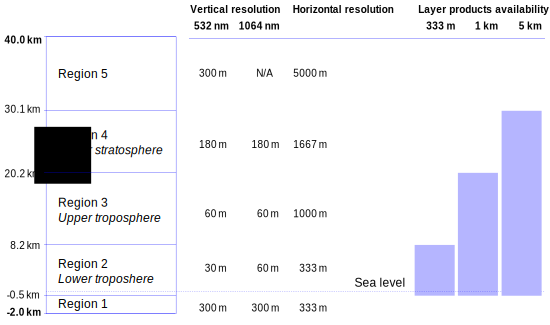
\includegraphics[width=380pt]{images/caliop-regions.pdf}
\caption[CALIOP regions]{\textbf{CALIOP regions.}
Typically, products based on CALIOP measurements cover the lowest
\SI{40}{km} of the atmosphere, separated logically into five regions based on
sampling resolution \citep{Winker2004}.}
\label{fig:caliop-regions}
\end{figure}

\section{CALIPSO}
The satellite CALIPSO (Cloud–Aerosol Lidar and Infrared Pathfinder Satellite
Observation) carries three nadir-viewing instruments that can be used to observe
properties of aerosols and micrometre-sized cloud particels: CALIOP lidar, IIR
imaging infrared radiometer, and a Wide Field Camera (WFC).

\subsection{CALIOP}
CALIOP (Cloud-Aerosol Lidar with Orthogonal Polarization) is a
polarisation-sensitive lidar capable of measuring backscatter intensity at
wavelengths of \SI{532}{nm}
and \SI{1064}{nm} at a repetition rate of \SI{20.16}{Hz}
\citep{CALIPSO_Catalog2007}. The primary products of this instrument are
vertical atmosphere profiles covering 5 vertical regions between \SI{-2.0}{km} 
and \SI{40.0}{km} (Fig.\,\ref{fig:caliop-regions}).

As you can see in Fig.\,\ref{fig:caliop}, the instrument's primary components
are a receiver and lasers mounted with a boresight mechanism. The Nd:YAG lasers
generate \SI{20}{nsec} pulses of \SI{110}{mJ} at two wavelengths: \SI{532}{nm}
and \SI{1064}{nm}. The bandwidth is \SI{30}{pm}, and polarisation purity is
1000:1. Emitted light is directed through beam expanders, which ensure
divergence of \SI{100}{{\textmu}rad}, i.e. a beam diameter of \SI{70}{m} on the
ground. The main components of the receiver subsystem are a 1-m-wide telescope
and three detectors --- one for the \SI{1064}{nm} channel and two for the
parallel and perpendicular polarisation of the \SI{532}{nm} channel
\citep{PC-SCI-202.01}.

\begin{figure}[t]
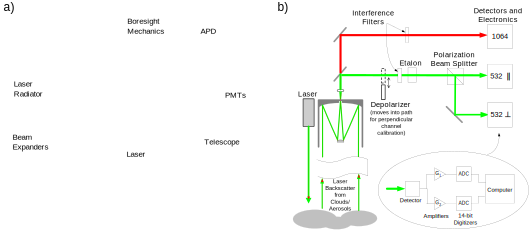
\includegraphics[width=\textwidth]{images/caliop.pdf}
\caption[CALIOP]{\textbf{CALIOP.} \textbf{a}, CALIOP transmitter and receiver
subsystems. \textbf{b}, Functional block diagram of CALIOP.
[Adapted from \cite{PC-SCI-201}.]}
\label{fig:caliop}
\end{figure}

\begin{table}
\caption[EOS processing levels]{\textbf{EOS processing levels.} Products from NASA EOS missions are
available in a number of levels depending on the amount of processing that has
been performed on raw data. A more detailed description is to be found
in \cite{EOS_DataProductsHandbook2004}.}
\label{tab:eos-levels}
\begin{tabularx}{\textwidth}{l X}
\sffamily{\textbf{Level}} &
\sffamily{\textbf{Description}}\\
\tophline
Level~0 &
Reconstructed, unprocessed instrument/payload data at full
resolution; any and all communications artifacts, e.g., synchronisation frames,
communications headers,
duplicate data removed.\\
Level~1A &
Reconstructed, unprocessed instrument data at full resolution,
time-referenced, and annotated with ancillary information, including radiometric
and geometric calibration coefficients and georeferencing parameters, e.g,
platform ephemeris, computed and appended but not applied to the Level~0
data.\\
Level~1B &
Level~1A data that have been processed to sensor units (not all
instruments have Level~1B data products).\\
Level~2
& Derived geophysical variables at the same resolution and location as
the Level~1 source data.\\
Level~3
& Variables mapped on uniform space-time grids, usually with some
completeness and consistency.\\
Level~4
& Model output or results from analyses of lower level data, e.g.,
variables derived from multiple measurements.
\end{tabularx}
\end{table}


\subsection{Data Products}\label{sec:calipso-data-products}
Data obtained by CALIPSO are processes by NASA LaRC (Langley Research Center)
into products and distributed as HDF (Hierarchical Data Format) files
to the scientific community. The products come in a set of levels depending on
the amount of processing that has been performed as defined by the
EOS guidelines (Tab.\,\ref{tab:eos-levels}). Each level of products originating from a
half-orbit
(day or night) is stored in a standalone HDF file.\\

\noindent\textit{The physical quantities used in the products description below are introduced in
Chapter\,\ref{chap:physical-basis}. Please read the relevant sections of this chapter
first if you are unfamiliar with the notation.}

\subsubsection{Lidar Instrument Level 1 Data Products}
\textit{Lidar Instrument Level 1 Data Products} contain data sets spanning
a vertical cross-section of the atmosphere. Values are stored
in rasters. Rows are associated with altitude, and columns are associated
with time, latitude and longitude (technically, the data sets are stored transposed,
but we like to think of columns as the vertical slices) . These products are processed to sensor units
and geolocated.
As of April 2010, Lidar Instrument Level 1 Data Products are available in the
\textit{Validated Stage 1}
maturity level (version 3.01), which means that `\textit{uncertainties are
estimated from independent measurements at selected locations and times}'
\citep{CALIPSO_QualityStatements}.
\pagebreak
\begin{description}
\item[Total Attenuated Backscatter 532nm]\hfill\\
The \textit{Total Attenuated Backscatter 532nm} is defined by the equation:
\begin{equation}
\beta_{532}' = \beta_{532} T_{532}^2 = (\beta_{532,\parallel} + \beta_{532,\perp}) T_{532}^2
\end{equation}
This are essentially the signals from the 532-nm parallel and perpendicular detectors combined,
calibrated and normalised to amplifier gain, laser energy and range (Section\,\ref{sec:caliop-the-fundamental-equation}\,).

\item[Perpendicular Attenuated Backscatter 532nm]\hfill\\
The \textit{Perpendicular Attenuated Backscatter 532nm} is the attenuated perpendicular component
of the 532-nm backscatter $\beta_{532,\perp}'$:
\begin{equation}
\beta_{532,\perp}' = \beta_{532,\perp} T_{532}^2
\end{equation}

\item[Attenuated Backscatter 1064nm]\hfill\\
The \textit{Attenuated Backscatter 1064nm} is $\beta_{1064}'$ as described in Chapter\,\ref{chap:physical-basis}.

\item[Attenuated Color Ratio]\hfill\\
The \textit{Attenuated Color Ratio} is defined by the equation:
\begin{equation}
\chi' = \frac{\beta_{1064}'}{\beta_{532}'}
\end{equation}
This data set is not contained within the Level 1 product files, but is calculated by \ccplot (Chapter\,\ref{chap:ccplot}).

\item[Depolarization Ratio]\hfill\\
The \textit{Depolarization Ratio} (at \SI{532}{nm}) is defined by the equation:
\begin{equation}
\delta = \frac{\beta_{532,\perp}}{\beta_{532,\parallel}} = \frac{\beta_{532,\perp}T_{532}^2}{\beta_{532,\parallel}T_{532}^2} = \frac{\beta_{532,\perp}'}{\beta_{532,\parallel}'}
\end{equation}
Note that since attenuation is the same for the perpendicular and parallel component of the 532-nm channel,
the depolarization ratio is in fact the same as the \textit{attenuated} depolarization ratio.

\end{description}


\subsubsection{Lidar Level 2 Cloud and Aerosol Layer Products}
\textit{Lidar Level 2 Cloud and Aerosol Layer Products} are higher-level
products that contain
scientific values integrated over vertical areas called \textit{layers},
associated with atmospheric features such as clouds and aerosols. Layers are
contained in a
procession of \textit{columns}. Column properties include the number of features
found within the column, and temporal and geospatial location. Layer properties
include layer top and base altitude, and physical properties of the feature such
as the \textit{Integrated Attenuated Backscatter} or the \textit{Integrated
Volume Depolarization Ratio}, some of which are described below. More
information can be found in
\cite{CALIPSO_QualityStatementsLidarLevel2CloudAndAerosolProfileProducts}.

As of April 2010, Lidar Level 2 Cloud and Aerosol Layer Products
are only available in the \textit{Provisional} maturity level (version 2.02),
which means that
`\textit{limited comparisons with independent sources have been made and obvious
artifacts fixed}' \citep{CALIPSO_QualityStatements}.

\begin{description}
\item[Integrated Attenuated Backscatter 532nm \& Integrated Attenuated
Backscatter 1064nm]\hfill
The \textit{Integrated Attenuated Backscatter} is computed by integrating
the attenuated backscatter coefficient
(\ref{eq:attenuated-backscatter})
due to particulates (with attenuations due to molecules and ozone removed) over a vertical path through the feature
\citep[Equation	\,3.11]{PC-SCI-202.02}:
\begin{equation}
\gamma'_{\lambda} = \int\limits_{top}^{base} \beta_{p,\lambda}(r) T^2_{p,\lambda}(r) \, \mathrm{d}r
\end{equation}
where $\lambda$ is either 532 or 1064 depending on wavelength.
%The values of $\gamma_{532}'$ are always corrected for attenuation impaired by
%any overlying features.
%The values $\gamma_{1064}'$ are \textit{not}.


\item[Integrated Attenuated Total Color Ratio 1064nm/532nm]\hfill\\
The \textit{Integrated Attenuated Total Color Ratio} is defined by the equation
\citep[Equation\,6.13]{PC-SCI-202.02}:
\begin{equation}
\chi' = \frac{\sum\limits_{k=top}^{base}
B_{1064}(z_k)}{\sum\limits_{k=top}^{base} B_{532}(z_k)}
\end{equation}
where $B_{\lambda}$ is the value of $\beta'_{\lambda}$ corrected for attenuation
by molecules and ozone (but not particles):
\begin{equation}
B_{\lambda} = \frac{\beta'_{\lambda}}{T^2_{m,\lambda} T^2_{O_3,\lambda}}
\end{equation}

\item[Integrated Volume Depolarization Ratio]\hfill\\
The \textit{Integrated Volume Depolarization Ratio} is defined by the equation
\citep[Equation\,6.10]{PC-SCI-202.02}:
\begin{equation}
\delta = \frac{\sum\limits_{k=top}^	{base}
\beta'_{532,\perp}(z_k)}{\sum\limits_{k=top}^{base} \beta'_{532,\parallel}(z_k)}
\end{equation}

\item[Midlayer Temperature]\hfill\\
This is the temperature in the geometric midpoint (vertically) of the layer derived from the GEOS-5 data product.
\end{description}

\begin{figure}[t]
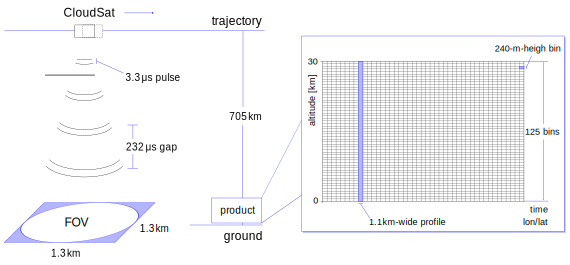
\includegraphics[width=\textwidth]{images/cloudsat-profile.pdf}
\caption[Scheme of CloudSat CPR operation]{\textbf{Scheme of CloudSat CPR operation.}
The radar sends 3.3-μm pulses at a rate of
\SI{4300}{Hz}. Pulses cover \SI{1.3}{km}\,\texttimes\,\SI{1.3}{km} instantaneous
footprint
on the ground, but the effective FOV is \SI{1.3}{km}\,\texttimes\,\SI{1.7}{km}.
Products
are generated for the lowest \SI{30}{km}. Profiles are sampled \SI{1.1}{km}
apart by averaging 688 pulses within \SI{0.16}{s}. Bins are sampled \SI{240}{m}
apart. Horizontal precision of profiles is \SI{1.7}{km}, vertical precision of
bins is \SI{500}{m}.}
\label{fig:cloudsat-profile}
\end{figure}

\section{CloudSat}\label{sec:atrain-cloudsat}
CloudSat is a NASA ESSP mission administered by the Colorado State University.
CloudSat is a `\textit{burdened}' satellite of the A-Train constellation, which means it
adjusts its position to be in a precise position with respect to CALIPSO and
Aqua, in order to overlap the footprint of instruments. The satellite carries a
single scientific instrument --- a nadir-viewing 94-GHz (3.2-mm wavelength) radar
called CPR (Cloud Profiling Radar), whose aim is to observe
vertical structure of clouds. CPR is similar in design to airborne cloud radars.
It operates by sending 3.3-μs pulses and measuring power backscattered by
cloud droplets or other hydrometeors as a function of distance. Pulses are
generated at PRF (Pulse Repetition Frequency) of \SI{4300}{Hz}, meaning two
consecutive pulses are \SI{232}{\micro s} apart. Only pluses backscattered from
up to
\SI{30}{km} from the ground are measured. Instantaneous FOV (Field of View) of a
pulse on the ground is approx. \SI{1.3}{km}. However, since a single profile is
produced by integrating 688 pulses over a period of \SI{0.16}{s}, the effective
FOV is elongated in the along-track direction to \SI{1.7}{km}. The primary
output of CPR is a vertical profile of the atmosphere
(Fig.\,\ref{fig:cloudsat-profile}).

\subsection{Data Products}
Measurements are down-linked, processed into products, and distributed by the
CloudSat Data Processing Centre as HDF-EOS2 files. Number of products are available
\citep{CloudSatHandbook2008}. Since the lowest-level product 1B-CPR does not contain
physical quantities suitable for immediate use by scientific applications, we will focus
on a higher-level product 2B-GEOPROF.

\subsubsection{2B-GEOPROF}
The \textit{2B-GEOPROF} product, also called the \textit{Cloud Geometrical Profile},
contains the primary useful physical quantity which can be calculated from
the received echo power --- Radar Reflectivity Factor \textit{$Z$}. Its value expresses
a relative attenuated backscatter strength as described in Section\,\ref{sec:cpr-physics}\, of \textit{The Physical Basis} chapter.
Radar Reflectivity Factor is comprised of 1.1-km-wide columns called \textit{rays} (or
\textit{profiles}), which are further composed of 125 240-m \textit{bins} in the vertical
direction. A single scientific value is assigned to each bin. All bins together
form a 2-dimensional raster on a 30-km-high irregular grid.
This product is available for both day and night granules \citep{1B-CPR_PDICD,2B-GEOPROF_PDICD,Stephens2002}.

\begin{table}[t]
\caption[MODIS bands]{\textbf{MODIS bands.}
Bands are organised in band groupings by their resolution.}
\label{tab:bands}
\begin{tabularx}{\textwidth}{llX}
  \sffamily{\textbf{Band grouping}}
& \sffamily{\textbf{Resolution}}
& \sffamily{\textbf{Bands}}\\
\tophline

EV\_250\_RefSB
& \SI{250}{m}
& 1, 2\\

EV\_500\_RefSB
& \SI{500}{m}
& 3, 4, 5, 6, 7\\

EV\_1KM\_RefSB
& \SI{1}{km}
& 8-12, 13lo, 13hi, 14lo, 14hi\mpfootnotemark[1], 15-19, 26\mpfootnotemark[2]\\

EV\_1KM\_Emissive
& \SI{1}{km}
& 20-25, 27-36
\end{tabularx}
\footnotetext[1]{Bands 13 and 14 are split into two sub-bands: high and low.}
\footnotetext[2]{Band 26 is exceptional in a sense that it is a
Reflective Solar Band in 1-km-resolution, and as such does not appear in night
mode granules (as thermal bands do).
Consequently, it is stored as a standalone SDS in HDF-EOS2 product files
in order to save space.}
\end{table}

\section{Aqua}
The NASA EOS mission satellite Aqua carries instruments predominantly used for
water cycle observation, but some of them also aid weather forecasting by
measuring temperature and humidity of the atmosphere, or the Earth Radiation
Budget. Aqua is one of the key EOS missions, the other being Terra, which 
complements Aqua in land observations
\citep{Parkinson2003}. There are six
instruments installed:

\begin{enumerate}
\item AIRS (Atmospheric Infrared Sounder)
\item AMSR-E (Advanced Microwave Scanning Radiometer - EOS)
\item AMSU (Advanced Microwave Sounding Unit)
\item CERES (Clouds and the Earth’s Radiant Energy System)
\item HSB (Humidity Sounder for Brazil)
\item MODIS (Moderate-Resolution Imaging Spectroradiometer)
\end{enumerate}

These instruments serve variety of purposes, and provide a very diverse range of
products \citep{ScienceWritersGuideToAqua2002}. We will confine our discussion
to the spectroradiometer MODIS.


\subsection{MODIS}
MODIS is a cross-track scanning radiometer administered by the MODIS Science
Team at NASA Goddard Space Flight Centre. Measurements are performed via the
means of a rotating scan mirror and an array
of detectors. The structure of its viewing swath is explained in
Fig.\,\ref{fig:modis-swath}. The spectroradiometer scans incident
radiation at 36 different visible and infrared channels at spatial resolution of
\SI{250}{m}, \SI{500}{m} and \SI{1}{km} depending on band
(Tab.\,\ref{tab:bands}). Bands 1--19 and 26
are reflective solar
bands (RSB) raging from \SI{0.405}{μm} to \SI{2.155}{μm}. Bands 20--25
and 27--36 are
thermal emissive bands (TEB) raging from \SI{3.66}{μm} to \SI{14.385}{μm} \cite{MODIS_Specifications}. A
large
number
of algorithms is employed to convert measured data into products related to
biosphere, oceans, atmosphere, land and cryosphere \citep{AquaBrochure2002}.
Total global coverage is completed within the course of two
days \citep{Xiong2006}.


\begin{figure}[t]
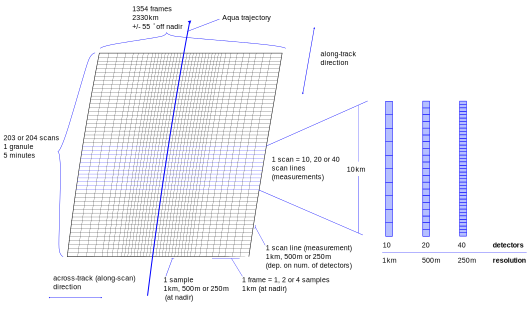
\includegraphics[width=400pt]{images/modis-swath.pdf}
\caption[Layout of a MODIS granule]{\textbf{Layout of a MODIS granule.} The observational swath is divided
into 5-min granules of 203 scans in the along-track direction. Field of view is
\ang{\pm55}
relative to nadir. The 250-m resolution bands have 40 detectors, the 500-m
resolution bands have 20 detectors and the 1-km-resolution bands have 10
detectors each. As indicated by the line density, resolution
decreases
with increasing distance from the trajectory.
A 10-km \textit{scan} of a mirror
comprises 10, 20 or 40 scan lines. Similarly, a 1-km \textit{frame} comprises 1,
2 or 4 \textit{samples}, depending on resolution.}
\label{fig:modis-swath}
\end{figure}

\subsection{Level~1B Data Products}\label{sec:modis-level1b-data-products}
MODIS products are categorised according to the EOS levels
(Tab.~\ref{tab:eos-levels}). Level~1B products are derived from Level 0 products
by calibration, geolocation and stripping into 5-minute swath granules.
These are then distributed in to form of HDF-EOS2 files through the EOS Data
Gateway.
Science Level~1B products are: \textbf{MYD02QKM} (250-m-resolution bands),
\textbf{MYD02HKM} (500-m-resolution bands and aggregated 250-m bands), and
\textbf{MYD021KM} (1-km-resolution bands and aggregated 250-m- and
500-m-resolution
bands). Documentation of MODIS products can be found
in \cite{MODIS_Level1B_ProductUsersGuide2009}.

\section{Data Ordering}
HDF4 and HDF-EOS2 data product files provided by CloudSat, CALIPSO and MODIS missions can be downloaded from the Internet through their
respective ordering systems:
\begin{itemize}
\item\textbf{CloudSat}. CloudSat products can be ordered from the \textit{CloudSat DPC} upon registration. Registration and ordering are free of charge.

\url{http://www.cloudsat.cira.colostate.edu}

\item\textbf{CALIPSO}. CALIPSO products can be ordered from \textit{Atmospheric Science Data Center} upon registration. Registration and ordering are free of charge.

\url{http://eosweb.larc.nasa.gov/PRODOCS/calipso/table_calipso.html}

\item\textbf{MODIS}. MODIS products are available through the \textit{LAADS Web} without registration. 

\url{http://ladsweb.nascom.nasa.gov}
\end{itemize}
